\documentclass[margin=0mm,tikz]{standalone}

\usepackage{tikz}
\usepackage{xcolor}

\usetikzlibrary{positioning}
\usetikzlibrary{fit}
\usetikzlibrary{calc}
\usetikzlibrary{arrows.meta}
\usetikzlibrary{quotes}
\usetikzlibrary{backgrounds}

\pgfdeclarelayer{background}
\pgfsetlayers{background,main}

% -----------------------
% colors
% -----------------------
\definecolor{polar1}{RGB}{180, 203, 231}
\definecolor{polar2}{RGB}{172, 192, 231}
\definecolor{equat1}{RGB}{231, 213, 168}
\definecolor{equat2}{RGB}{231, 203, 173}

% Set background color
%\pagecolor{white}


\tikzstyle{p1face} = [
    draw=black,
    top color = polar1,
    bottom color = polar1,
    minimum size=1.5cm,
    rotate=-45
]
\tikzstyle{p2face} = [
	draw=black,
	top color = polar2,
	bottom color = polar2,
	minimum size=1.5cm,
	rotate=-45
]
\tikzstyle{e1face} = [
	draw=black,
	top color = equat1,
	bottom color = equat1,
	minimum size=1.5cm,
	rotate=-45
]
\tikzstyle{e2face} = [
	draw=black,
	top color = equat2,
	bottom color = equat2,
	minimum size=1.5cm,
	rotate=-45
]
\tikzstyle{nface} = [
	draw=black,
	top color = blue!20!white,
	bottom color = blue!30!white,
	minimum size=1.5cm,
	opacity=0.5,
	rotate=-45
]
\tikzstyle{diag} = [
	dotted,
	opacity=0.5
]

% Box with different colors, modified from
% https://tex.stackexchange.com/questions/343354/tikz-rectangle-with-diagonal-fill-two-colors
\tikzset{
	diagonal fill/.style 2 args={
		path picture={
			\fill[#1] (path picture bounding box.south) -| (path picture bounding box.north) -- cycle;
			\fill[#2] (path picture bounding box.north) -| (path picture bounding box.south) -- cycle;
		}
	},
}


\begin{document}
	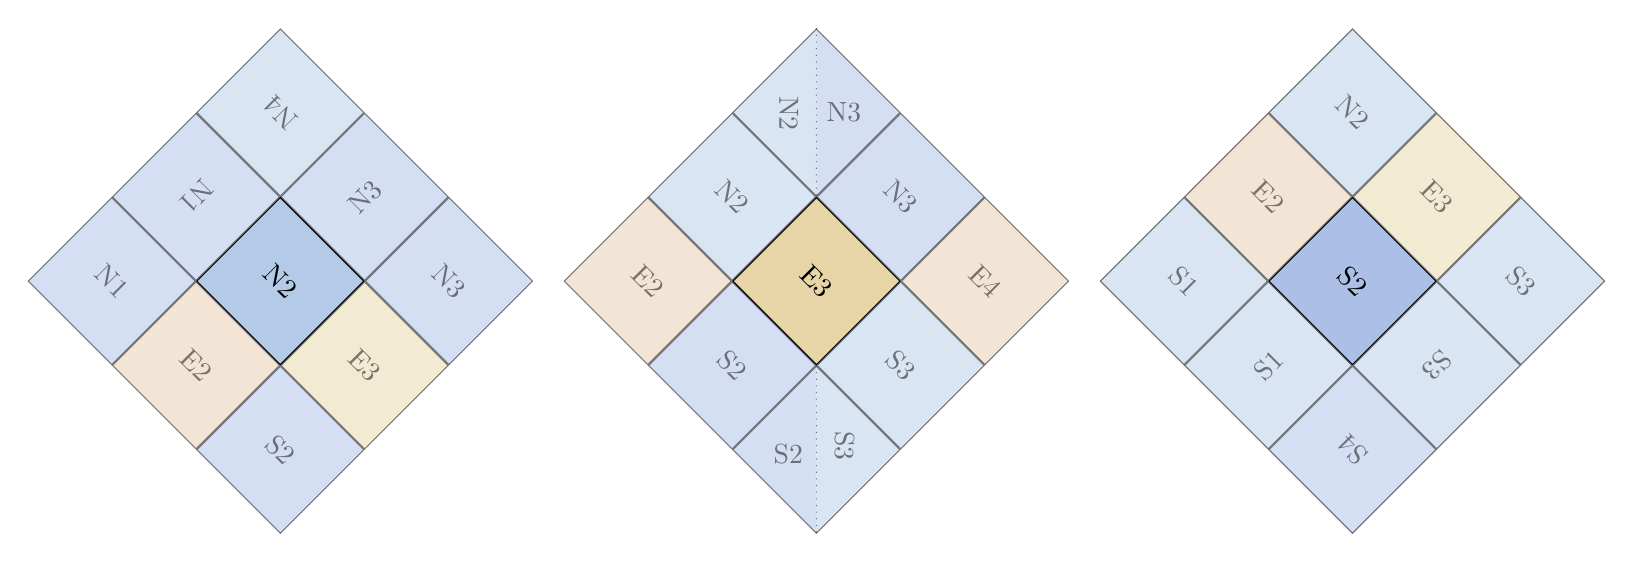
\begin{tikzpicture}[node distance=0cm and 0cm]
	
	% North face
	\node[p1face] (N2) {N2};
	\node[p2face, opacity=0.5, above=of N2] {\rotatebox{90}{N3}};
	\node[p1face, opacity=0.5, above left=of N2] {\rotatebox{180}{N4}};
	\node[p2face, opacity=0.5, left=of N2] {\rotatebox{270}{N1}};
	\node[p2face, opacity=0.5, below left=of N2] {N1};
	\node[e2face, opacity=0.5, below=of N2] {E2};
	\node[p2face, opacity=0.5, below right=of N2] {S2};
	\node[e1face, opacity=0.5, right=of N2] {E3};
	\node[p2face, opacity=0.5, above right=of N2] {N3};
	
	% Equator faces
	\node[e1face, above right=of N2, xshift=3.3cm, yshift=3.3cm] (E3) {E3};
	\node[p2face, opacity=0.5, above=of E3] {N3};
	\node[diagonal fill={polar1}{polar2}, opacity=0.5, minimum size=1.5cm, draw, rotate=-45, above left=of E3] (E3nw) {\rotatebox[origin=c,x=-0.5cm]{-45}{N2}\rotatebox[origin=c]{45}{N3}};
	\draw[diag] (E3nw.north west)--(E3nw.south east);
	\node[p1face, opacity=0.5, left=of E3] {N2};
	\node[e2face, opacity=0.5, below left=of E3] {E2};
	\node[p2face, opacity=0.5, below=of E3] {S2};
	\node[diagonal fill={polar2}{polar1}, opacity=0.5, minimum size=1.5cm, draw, rotate=-45, below right=of E3] (E3se) {\rotatebox[origin=c, x=1cm]{45}{S2}\rotatebox[origin=c]{-45}{S3}};
	\draw[diag] (E3se.north west)--(E3se.south east);
	\node[p1face, opacity=0.5, right=of E3] {S3};
	\node[e2face, opacity=0.5, above right=of E3] {E4};
	
	% South face
	\node[p2face, above right=of E3, xshift=3.3cm, yshift=3.3cm] (S2) {S2};
	\node[e1face, opacity=0.5, above=of S2] {E3};
	\node[p1face, opacity=0.5, above left=of S2] {N2};
	\node[e2face, opacity=0.5, left=of S2] {E2};
	\node[p1face, opacity=0.5, below left=of S2] {S1};
	\node[p1face, opacity=0.5, below=of S2] {\rotatebox{90}{S1}};
	\node[p2face, opacity=0.5, below right=of S2] {\rotatebox{180}{S4}};
	\node[p1face, opacity=0.5, right=of S2] {\rotatebox{270}{S3}};
	\node[p1face, opacity=0.5, above right=of S2] {S3};
		
	\end{tikzpicture}
\end{document}